\chapter{Analyse van de reslutaten}%
\label{ch:analyse}

\section{Nauwkeurigheid MQ-sensoren}
\label{sec:nauwkeurigheid}

\subsection{Ammoniak (NH\textsubscript{3})}
\label{subsec:nh3}

TODO


\subsection{Koolstofdioxide (CO\textsubscript{2})}
\label{subsec:co2}

TODO (de CO2 test gaat aanstaande woensdag door)

\section{Analyse van de warmte-koelcyclus}
\label{sec:analyse_mq7}

Zoals reeds aangehaald in sectie~\ref{sec:warmte_koel} is de warmte-koelcyclus getest in een normale omgeving, dit was buiten, en een omgeving met een hoge luchtvochtigheid, dit was een dampige badkamer. Zo zijn er per omgeving 3 gassen getest: alcohol, CO en LPG. De resultaten werden in de databank opgeslagen en gevisualiseerd in PowerBI. De resultaten zijn te zien op de volgende figuren, waarbij de blootstelling aan het specifieke gas in het rood staat gekleurd.

\begin{figure}[h!]
    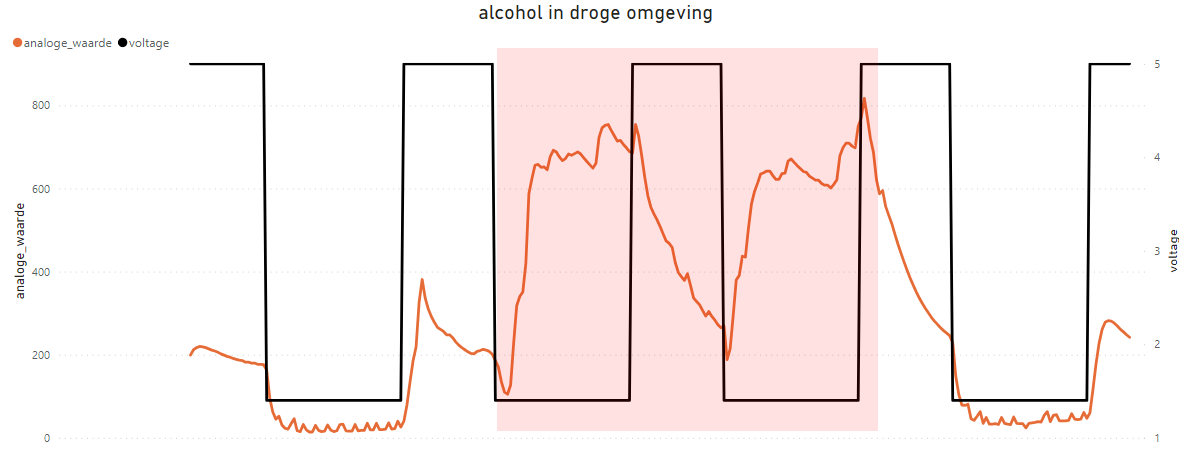
\includegraphics[scale=0.65, center]{alcohol_droog.png}
    \caption[Alcohol in droge omgeving]{Alcohol in droge omgeving}
    \label{fig:alcohol_droog}
\end{figure}

\begin{figure}[h!]
    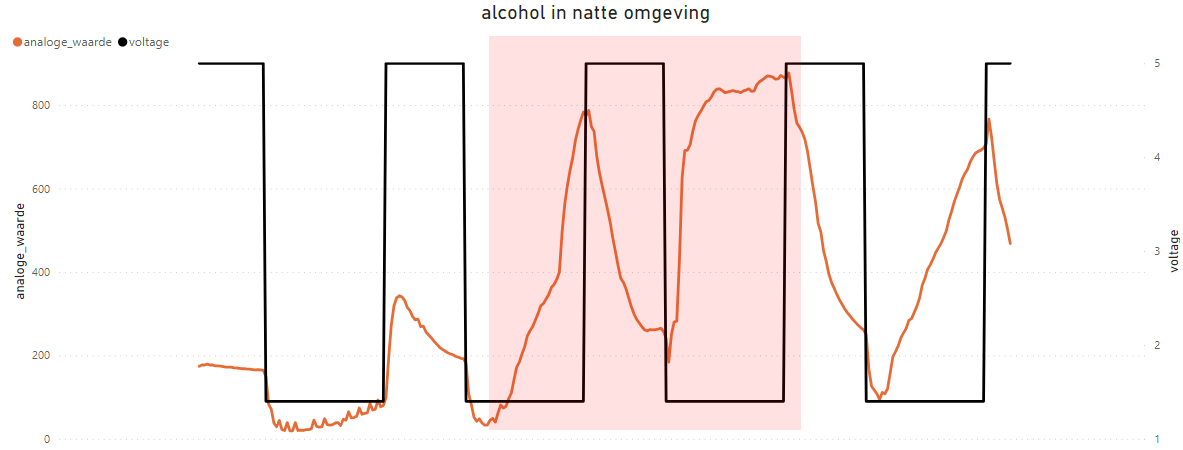
\includegraphics[scale=0.65, center]{alcohol_nat.png}
    \caption[Alcohol in natte omgeving]{Alcohol in natte omgeving}
    \label{fig:alcohol_nat}
\end{figure}

\begin{figure}[h!]
    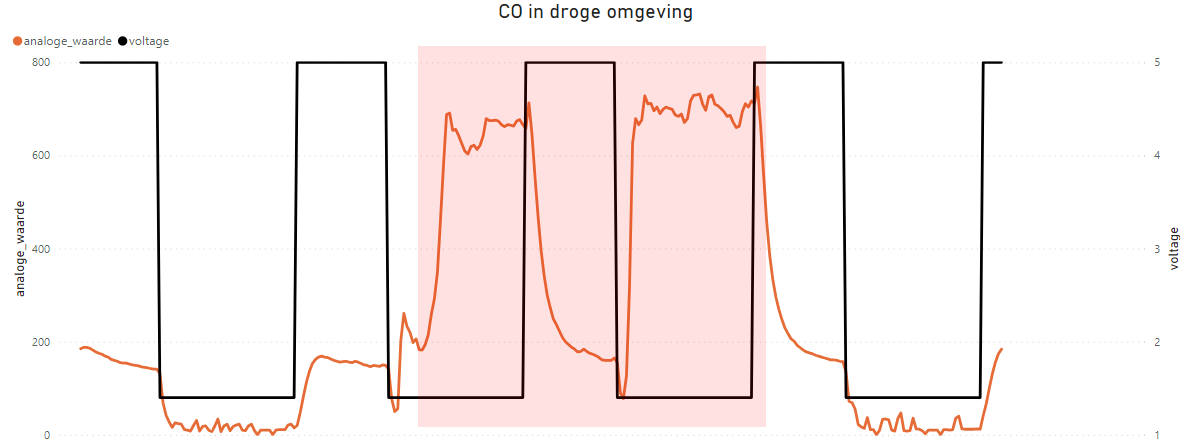
\includegraphics[scale=0.65, center]{co_droog.png}
    \caption[CO in droge omgeving]{CO in droge omgeving}
    \label{fig:co_droog}
\end{figure}

\begin{figure}[h!]
    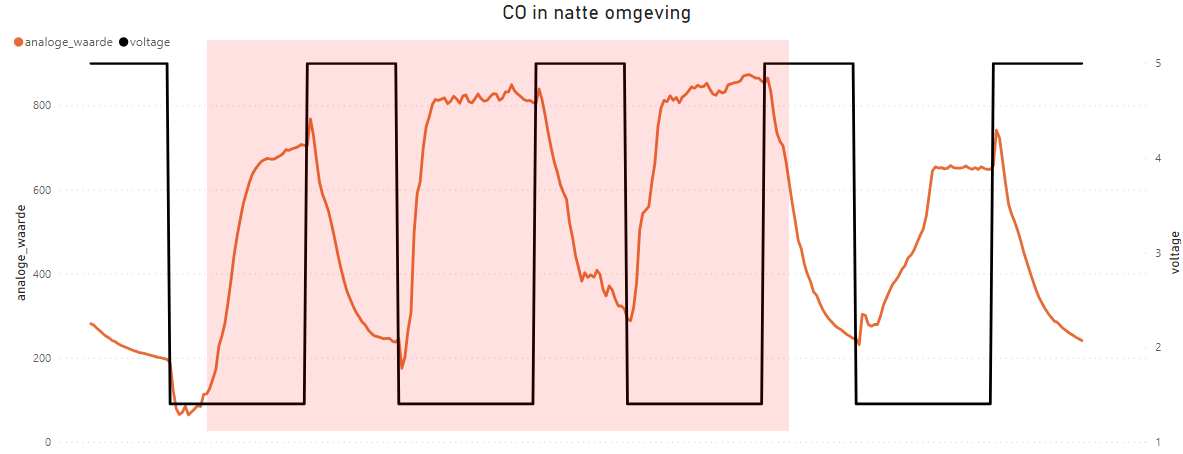
\includegraphics[scale=0.65, center]{co_nat.png}
    \caption[CO in natte omgeving]{CO in natte omgeving}
    \label{fig:co_nat}
\end{figure}

\begin{figure}[h!]
    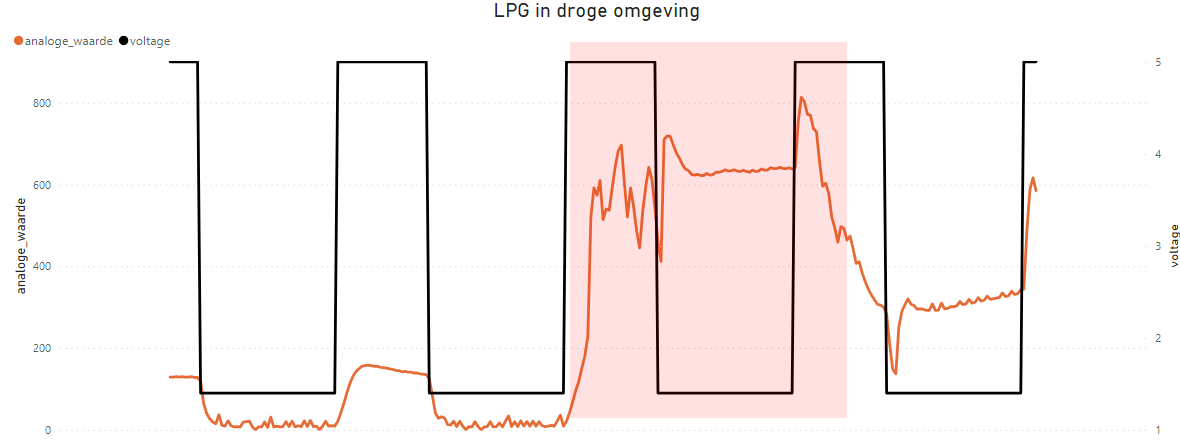
\includegraphics[scale=0.65, center]{lpg_droog.png}
    \caption[LPG in droge omgeving]{LPG in droge omgeving}
    \label{fig:lpg_droog}
\end{figure}

\begin{figure}[h!]
    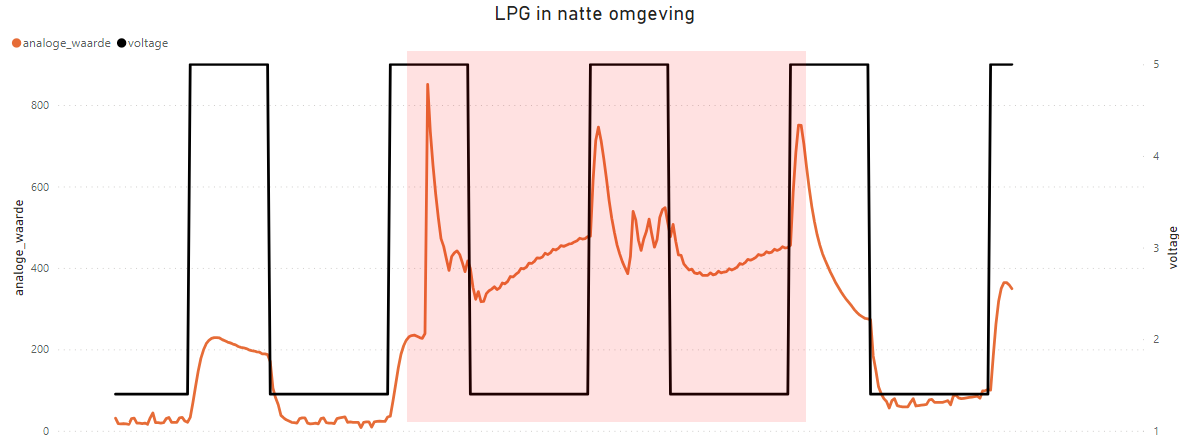
\includegraphics[scale=0.65, center]{lpg_nat.png}
    \caption[LPG in natte omgeving]{LPG in natte omgeving}
    \label{fig:lpg_nat}
\end{figure}


%\pagebreak
\clearpage
\subsection{Invloed van luchtvochtigheid}
\label{subsec:invloed_hum}

Op de resultaten is te zien dat de luchtvochtigheid wel degelijk een rol speelt bij de lezingen van de MQ-7 sensor. 

Het eerste wat opvalt is dat zowel bij alcohol (\ref{fig:alcohol_droog} \&~\ref{fig:alcohol_nat}) als CO (\ref{fig:co_droog} \&~\ref{fig:co_nat}) de waarde hoger is in een vochtige omgeving dan in een normale omgeving, terwijl voor LPG (\ref{fig:lpg_droog} \&~\ref{fig:lpg_nat}) juist het omgekeerde geldt. Dit verschijnsel kan worden verklaart met het feit dat stoffen homo- en heterogeen kunnen zijn.
Door de vochtige omgeving zit de sensor vol met watermoleculen. Doordat water en LPG sterk heterogeen zijn, en dus net als water en olie niet kunnen worden gemengd, zal deze sensor bij aanraking met LPG een minder hoge waarde uitlezen als normaal. Omdat CO juist homogeen is zijn de waarden hier hoger dan normaal. Bij alcohol kan de mengbaarheid afhangen van de soort alcohol, in dit geval is er ontsmettingsalcohol gebruikt die volgens de deze redenering dus ook homogeen blijkt te zijn met water.

Bij zowel alcohol als CO zijn er weinig verschillen in de droge- en natte grafieken, naast dat de waarde hoger wordt dan normaal en iets stabieler is in de koelfase. Maar bij LPG is er een duidelijker verschil te zien in de koelfase. Zo stabiliseert de waarde vrij snel in de droge omgeving (\ref{fig:lpg_droog}), terwijl ze in natte omgeving (\ref{fig:lpg_nat}) juist heel geleidelijk aan toeneemt.


\subsection{Onderscheiden van verschillende gassen}
\label{subsec:onderscheiding_gassen}


Omdat elk soort gas zich anders gedraagt zouden deze onderscheidbaar moeten kunnen zijn op de grafieken. Zo valt meteen de grafiek van CO op (\ref{fig:co_droog}). De MQ-7 sensor is het meest gevoelig voor CO en op de grafiek is dan ook merkbaar hoe snel de waarde klimt wanneer de sensor wordt blootgesteld aan CO. Ook zal de CO het snelste worden weggedreven door een hoge temperatuur.

Alcohol (\ref{fig:alcohol_droog}) klimt daarentegen trager en is veel minder stabiel, waardoor de uiteindelijke lezing na de koelcyclus minder kan accuraat zijn.

LPG heeft de meest merkbare grafiek (\ref{fig:lpg_droog}), zo is te zien hoe LPG zeer stabiel is in de koelcyclus. En tijdens de warmtecyclus een minder grote dip neemt dan de andere gassen. 

Hieruit kan worden opgemerkt dat MQ-7 sensor minder gevoelig is voor alcohol dan LPG en CO. Dit wordt ook aangetoond in de gevoeligheidscurve van de MQ-7 datasheet
%TODO bron datasheet mq7
te zien in figuur~\ref{fig:MQ7_grafiek}.

\begin{figure}[h]
    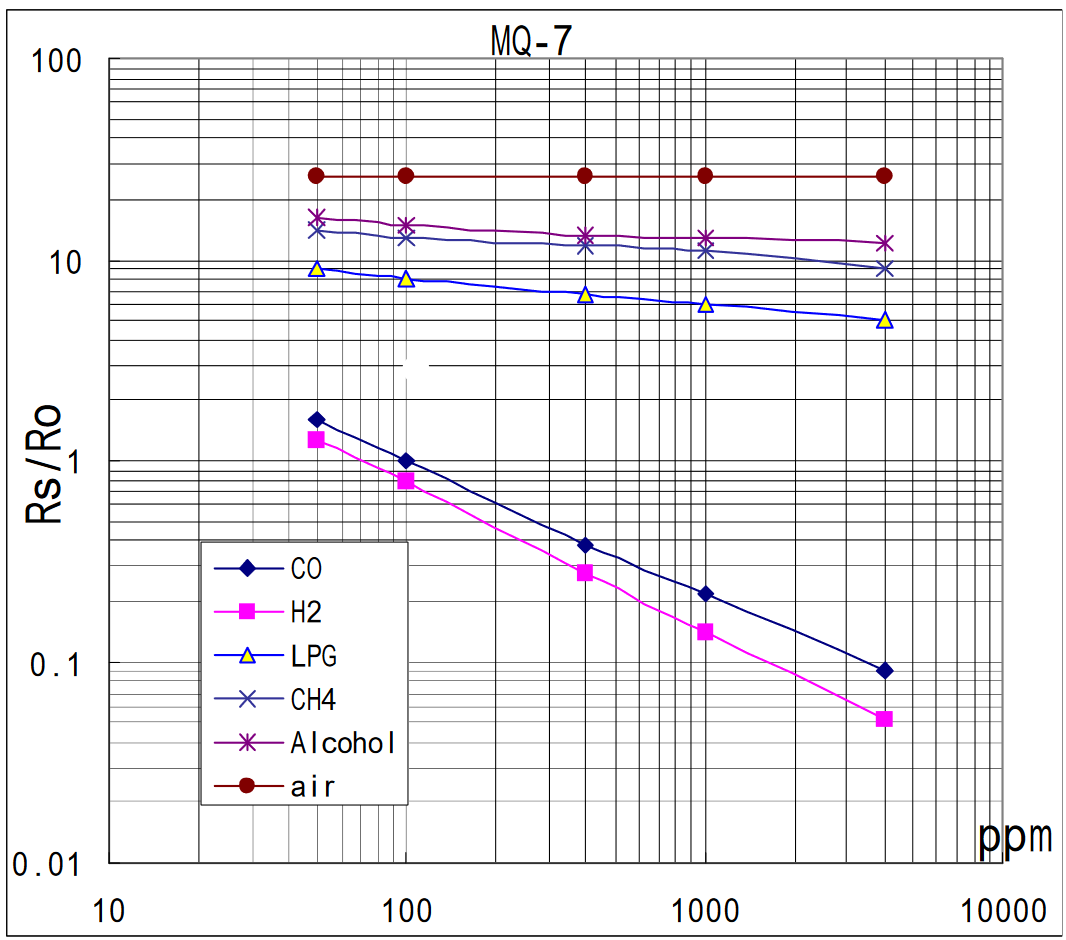
\includegraphics[scale=0.4, center]{MQ7_grafiek.png}
    \caption[Gevoeligheidscurve MQ-7]{Gevoeligheidscurve van de MQ-7 sensor
        %TODO bron datasheet mq135
    }
    \label{fig:MQ7_grafiek}
\end{figure}













